\documentclass[../main-sheet.tex]{subfiles}
\usepackage{../style}
\graphicspath{ {../img/} }
\backgroundsetup{contents={}}
\begin{document}
\chapter{Non-Linear Programming}
\section{Preliminary Concepts}
Let a model be
\begin{maxi*}
    {}{Z=f(x_1,x_2,\dots,x_n)}{}{}
    \addConstraint{g^1(x_1,x_2,\dots,x_n)}{\quad\{\leq,\text{ or } = \text{ or }\geq\} \quad b_1}
    \addConstraint{g^2(x_1,x_2,\dots,x_n)}{\quad\{\leq,\text{ or } = \text{ or }\geq\} \quad b_2}
    \addConstraint{\vdots\qquad\quad}{\qquad\vdots}
    \addConstraint{g^m(x_1,x_2,\dots,x_n)}{\quad\{\leq,\text{ or } = \text{ or }\geq\}\quad b_m}
    \addConstraint{x_i}{\geq0\qquad i=1,2,\dots,n}
\end{maxi*}
If \(f\) or \(g^i\) or both of them have one or more non-linear expression (i.e., have a variable that has degree 2 or above)  then this type of problems are called non-linear programming problem.\\
Matrix form
\begin{maxi*}
    {}{Z=f(\underline{x})}{}{}
    \addConstraint{g^i(\underline{x})}{\quad \{\leq,\text{ or } = \text{ or }\geq\}\quad b_i\qquad i=1,2,\dots,m}
    \addConstraint{\Rightarrow h^i(\underline{x})}{\quad \{\leq,\text{ or } = \text{ or }\geq\} \quad 0 \qquad \text{where }h^i(\underline{x})=g^i(\underline{x})-b_i}
\end{maxi*}
\subsection{Principal minor} Let \(Q_{n\times n}\) a matrix. It's \(k\)-th order \((k\leq n)\) principal minor is a matrix that is obtained from \(Q\) by removing \((n-k)\) corresponding rows and column.\\
Let
\[A=\begin{pmatrix}
    1&2&3\\
    4&5&6\\
    7&8&9
\end{pmatrix}
\]
its principal minors are
\begin{align*}
    \text{Order }1:&\begin{pmatrix}
        1
    \end{pmatrix},\,\begin{pmatrix}
        5
    \end{pmatrix},\,\begin{pmatrix}
        9
    \end{pmatrix}\\
    \text{Order }2:&\begin{pmatrix}
        1 & 2\\
        4&5
    \end{pmatrix},\,\begin{pmatrix}
        1& 3\\
        7&9
    \end{pmatrix},\,\begin{pmatrix}
        5&6\\
        8&9
    \end{pmatrix}\\
    \text{Order }3:&\begin{pmatrix}
        1&2&3\\
    4&5&6\\
    7&8&9
    \end{pmatrix}
\end{align*}
\emph{Leading principal minor}: Remove last \(n-k\) corresponding row and column.\\
\emph{Principal determinant}:
\begin{align*}
    \text{Order }1:&\begin{vmatrix}
        1
    \end{vmatrix},\,\begin{vmatrix}
        5
    \end{vmatrix},\,\begin{vmatrix}
        9
    \end{vmatrix}\\
    \text{Order }2:&\begin{vmatrix}
        1 & 2\\
        4&5
    \end{vmatrix},\,\begin{vmatrix}
        1& 3\\
        7&9
    \end{vmatrix},\,\begin{vmatrix}
        5&6\\
        8&9
    \end{vmatrix}\\
    \text{Order }3:&\begin{vmatrix}
        1&2&3\\
    4&5&6\\
    7&8&9
    \end{vmatrix}
\end{align*}
\subsection{Quadratic form} \(Q(x)=\sum_{i=0}^n \sum_{j=0}^n\,a_{ij}x_ix_j\)\\
e.g., \(Q(x)=x_1^2+7x_2^2+2x_3^2+2x_1x_2+4x_1x_3+6x_2x_3\) is a quadratic form because every term has degree of two.\\
\[\begin{pmatrix}
    x_1 & x_2 & x_3
\end{pmatrix}\,\begin{pmatrix}
    1& 0&1\\
    2& 7&6\\
    3& 0&2
\end{pmatrix}=\begin{pmatrix}
    x_1+2x_2+3x_3 & 7x_2 & x_1+6x_2+2x_3
\end{pmatrix}\]
\[\begin{pmatrix}
    x_1 & x_2 & x_3
\end{pmatrix}\,\begin{pmatrix}
    1& 0&1\\
    2& 7&6\\
    3& 0&2
\end{pmatrix}\begin{pmatrix}
    x_1\\
    x_2\\
    x_3
\end{pmatrix}=x_1^2+7x_2^2+2x_3^2+2x_1x_2+4x_1x_3+6x_2x_3
\]
So, \(Q(x)=\sum_{i=0}^n \sum_{j=0}^n\,a_{ij}x_ix_j=\mathbf{X}^T\mathbf{A\,X}\) (here \(\mathbf{A}\) can be symmetric) where \(\mathbf{X}=\begin{pmatrix}
    x_1\\
    x_2\\
    x_3
\end{pmatrix}\)\\
Again,
\[\begin{pmatrix}
    x_1 & x_2 & x_3
\end{pmatrix}\,\begin{pmatrix}
    1& 1&2\\
    1& 7&3\\
    2& 3&2
\end{pmatrix}\begin{pmatrix}
    x_1\\
    x_2\\
    x_3
\end{pmatrix}=x_1^2+7x_2^2+2x_3^2+2x_1x_2+4x_1x_3+6x_2x_3
\]
The quadratic form \(Q(x)=\mathbf{X}^T\mathbf{A\,X}\) is said to be
\begin{enumerate}
    \item Positive definite: if \(Q(x)>0\,\forall \underline{x}\neq 0\)
    \item Positive semi-definite: if \(Q(x)\geq 0\) for all \(x\) such that there exists at least one \(x\neq 0\) satisfying \(Q(x)=0\)
    \item Negative definite: \(-Q(x)>0\) or \(Q(x)<0\)
    \item Negative semi-definite: \(-Q(x)\geq0\) or \(Q(x)\leq 0\)
    \item Indefinite: if quadratic form does not fall into above categories.
\end{enumerate}
\begin{ex}\hfill
    \begin{itemize}
        \item Positive definite: \(Q(x)=3x_1^2+2x_2^2+x_3^2\)
        \item Positive semi-definite: \(Q(x)=(x_1-x_2)^2+2x_3^2\) \(x_1=x_2\) and \(x_3=0\)
        \item Negative definite: \(Q(x)=-x_1^2-3x_2^2\)
        \item Indefinite: \(Q(x)=x_1^2-3x_2^2\)
    \end{itemize}
\end{ex}
\emph{The necessary and sufficient condition:}
\begin{enumerate}
    \item Positive definite: \(Q(x)=\mathbf{X}^T\mathbf{A\,X}\) if leading principal determinant \(>0\)
    \item Positive semi-definite: \(Q(x)=\mathbf{X}^T\mathbf{A\,X}\) if leading principal determinant \(\geq 0\)
    \item Negative definite: \(Q(x)=\mathbf{X}^T\mathbf{A\,X}\) if sign of \(k-\)th leading principal determinant \(=(-1)^k\)
    \item Negative semi-definite: \(Q(x)=\mathbf{X}^T\mathbf{A\,X}\) if sign of \(k-\)th leading principal determinant \(=(-1)^k\) or zero
    \item Indefinite: there must be two opposite sign in diagonal.
\end{enumerate}
\begin{ex}
    \(Q(x)=2x_1^2+2x_2^2+3x_3^2+2x_1x_2+2x_2x_3\)\\
    Here, \(A=\begin{pmatrix}
        2&2&0\\
        0&2&2\\
        0&0&3
    \end{pmatrix}\)\\
    The leading principal determinants of \(A\): \(\begin{vmatrix}
        2
    \end{vmatrix}=2\), \(\begin{vmatrix}
        2&2\\
        0&2
    \end{vmatrix}=4\), \(\begin{vmatrix}
        2&2&0\\
        0&2&2\\
        0&0&3
    \end{vmatrix}=12\)\\
    So \(Q(x)\) is positive definite.
\end{ex}
\subsection{Hessian matrix:} Let \(f(\underline{x})=f(x_1,x_2,\dots,x_n)\) be a function that is continuous has double derivative. Then Hessian matrix of \(f(\underline{x})\) is \(H(\underline{x})=\begin{pmatrix}
        \dfrac{\partial^2 f}{\partial x_1^2} & \dfrac{\partial^2 f}{\partial x_1\,\partial x_2} & \cdots & \dfrac{\partial^2 f}{\partial x_1\,\partial x_n} \\[2.2ex]
        \dfrac{\partial^2 f}{\partial x_2\,\partial x_1} & \dfrac{\partial^2 f}{\partial x_2^2} & \cdots & \dfrac{\partial^2 f}{\partial x_2\,\partial x_n} \\[2.2ex]
        \vdots & \vdots & \ddots & \vdots \\[2.2ex]
        \dfrac{\partial^2 f}{\partial x_n\,\partial x_1} & \dfrac{\partial^2 f}{\partial x_n\,\partial x_2} & \cdots & \dfrac{\partial^2 f}{\partial x_n^2}
\end{pmatrix}\)\\
    \[f(x_1,x_2,x_3)=\begin{pmatrix}
        \dfrac{\partial^2 f}{\partial x_1^2} & \dfrac{\partial^2 f}{\partial x_1\,\partial x_2} & \dfrac{\partial^2 f}{\partial x_1\,\partial x_3} \\[2.2ex]
        \dfrac{\partial^2 f}{\partial x_2\,\partial x_1} & \dfrac{\partial^2 f}{\partial x_2^2} & \dfrac{\partial^2 f}{\partial x_2\,\partial x_3} \\[2.2ex]
        \dfrac{\partial^2 f}{\partial x_3\,\partial x_1} & \dfrac{\partial^2 f}{\partial x_3\,\partial x_2} & \dfrac{\partial^2 f}{\partial x_3^2}
      \end{pmatrix}
      \]
      Hessian matrix is a symmetric matrix [\(\because f_{ij}=f_{ji}\)].
      \begin{prob}
          Find the Hessian matrix of \(f(x,y)=x^3-2xy-y^6\) at the point \((1,2)\)
      \end{prob}
      \begin{soln}\hfill

          \(\qquad\dfrac{\partial f}{\partial x}=3x^2-2y\)
          \(\qquad\dfrac{\partial^2 f}{\partial x^2}=6x\)
          \(\qquad\dfrac{\partial f}{\partial x \,\partial y}=-2\)
          \(\qquad\dfrac{\partial f}{\partial y \,\partial x}=-2\)
          \(\qquad\dfrac{\partial^2 f}{\partial y^2}=-30y^4\)
          \begin{align*}
            H&=\begin{pmatrix}
                6x&-2\\
                -2&-30y^4
            \end{pmatrix}\\
            H_{(1,2)}&=\begin{pmatrix}
                6&-2\\
                -2&-480
            \end{pmatrix}
        \end{align*}
      \end{soln}
\subsection{Convex and concave function:} If \(f[\lambda x_1+(1-\lambda) x_2]\leq \lambda f(x_1)+(1-\lambda) f(x_2)\) where \(x_1\), \(x_2\) are points and \(0\leq\lambda\leq1\), then \(f(x)\) is a convex function. \(f(x)\) is strictly convex if \(f[\lambda x_1+(1-\lambda) x_2]< \lambda f(x_1)+(1-\lambda) f(x_2)\) where \(0<\lambda<1\).
\begin{figure}[H]
    \centering
    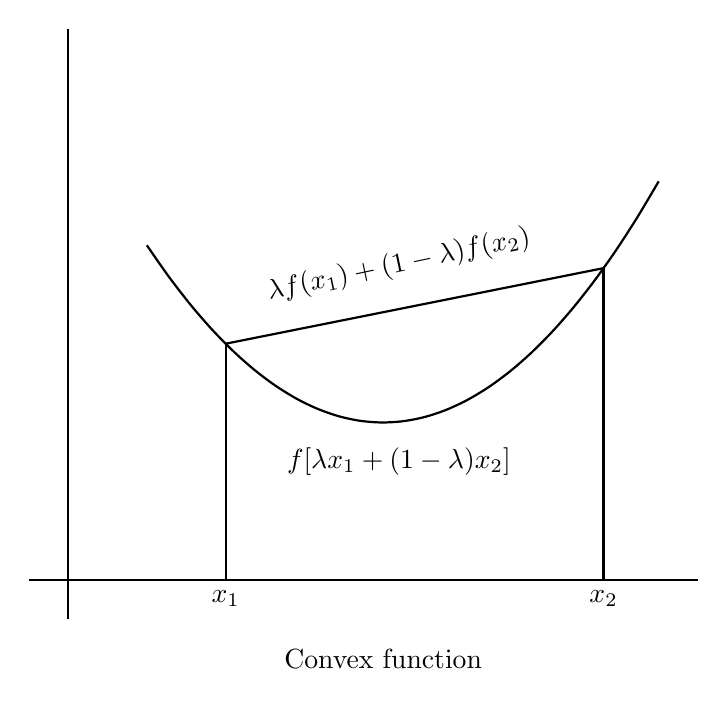
\begin{tikzpicture}
        \draw[thick,domain=1:7.5,smooth,variable=\x] plot (\x,{2+((0.5*\x)-2)^2});
        \draw[thick] (-0.5,0)--(8,0);
        \draw[thick](0,-0.5)--(0,7);
        \draw[thick](2,0)node [below]{$x_1$}--(2,3);
        \draw[thick](6.8,0)node [below] {$x_2$}--(6.8,3.96);
        \draw[thick](2,3)--(6.8,3.96);
        \node[rotate=12] at (4.2,4) {$\lambda f(x_1)+(1-\lambda)f(x_2)$};
        \node[rotate=0] at (4.2,1.5) {$f[\lambda x_1+(1-\lambda)x_2]$};
        \node at (4,-1) {Convex function};
    \end{tikzpicture}
    \qquad
    % \vspace{2cm}
    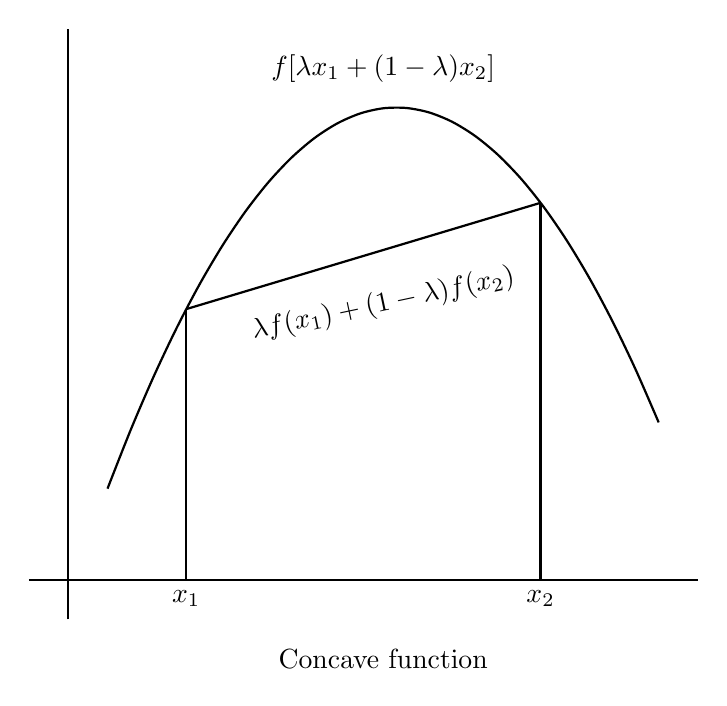
\begin{tikzpicture}
            \draw[thick,domain=0.5:7.5,smooth,variable=\x] plot (\x,{6-((0.6*\x)-2.5)^2});
            \draw[thick] (-0.5,0)--(8,0);
            \draw[thick](0,-0.5)--(0,7);
            \draw[thick](1.5,0)node [below]{$x_1$}--(1.5,3.44);
            \draw[thick](6,0)node [below] {$x_2$}--(6,4.79);
            \draw[thick](1.5,3.44)--(6,4.79);
            \node[rotate=12] at (4,3.5) {$\lambda f(x_1)+(1-\lambda)f(x_2)$};
            \node[rotate=0] at (4,6.5) {$f[\lambda x_1+(1-\lambda)x_2]$};
            \node at (4,-1) {Concave function};
        \end{tikzpicture}
\end{figure}
If \(f[\lambda x_1+(1-\lambda) x_2]\geq \lambda f(x_1)+(1-\lambda) f(x_2)\) where \(x_1\), \(x_2\) are points and \(0\leq\lambda\leq1\), then \(f(x)\) is a concave function. \(f(x)\) is strictly concave if \(f[\lambda x_1+(1-\lambda) x_2]> \lambda f(x_1)+(1-\lambda) f(x_2)\) where \(0<\lambda<1\).\\
\emph{Tests for a function to be convex/concave:} \(H(x)\) is the Hessian matrix of \(f(x)\)
\begin{itemize}
    \item Convex: if \(H(x)\) is positive semi-definite
    \item Strictly convex: if \(H(x)\) is positive definite
    \item Concave: if \(H(x)\) is negative semi-definite
    \item Strictly concave: if \(H(x)\) is negative definite
\end{itemize}
\begin{prob}
    Test the convexity of the function \(f(\underline{x})=3x_1^2+2x_2^2+x_3^2-2x_1x_2-2x_1x_3-6x_1-4x_2-2x_3\) at the point \((x_1,\,x_2,\,x_3)\).
\end{prob}
\begin{soln}
    The given function is \(f(\underline{x})=3x_1^2+2x_2^2+x_3^2-2x_1x_2-2x_1x_3-6x_1-4x_2-2x_3\)
    \begin{table}[H]
        \centering
        \begin{tabular}{l@{\quad}|@{\quad}l@{\quad}|@{\quad}l}
            \(\dfrac{\partial f}{\partial x_1}=6x_1-2x_2-2x_3-6\)&\(\dfrac{\partial^2 f}{\partial x_1^2}=6\)&\(\dfrac{\partial^2 f}{\partial x_1\,\partial x_2}=-2=\dfrac{\partial^2 f}{\partial x_2\,\partial x_1}\)\\[2.5ex]
            \(\dfrac{\partial f}{\partial x_2}=4x_2-2x_1+2x_3-4\)&\(\dfrac{\partial^2 f}{\partial x_2^2}=4\)&\(\dfrac{\partial^2 f}{\partial x_1\,\partial x_3}=-2=\dfrac{\partial^2 f}{\partial x_3\,\partial x_1}\)\\[2.5ex]
            \(\dfrac{\partial f}{\partial x_3}=3x_3-2x_1+2x_2-2\)&\(\dfrac{\partial^2 f}{\partial x_3^2}=2\)&\(\dfrac{\partial^2 f}{\partial x_2\,\partial x_3}=2=\dfrac{\partial^2 f}{\partial x_3\,\partial x_2}\)\\
        \end{tabular}
    \end{table}
    Then the Hessian matrix of the function \(f(x)\) is
    \[H(\underline{x})=\begin{pmatrix}
        6&-2&-2\\
        -2&4&2\\
        -2&2&2
    \end{pmatrix}
    \]
    Since,
    \begin{enumerate}[label=(\roman*)]
        \item \(H(\underline{x})\) is symmetric
        \item All diagonal elements are positive
        \item The leading principal minor determinant \(\begin{vmatrix}
            6
        \end{vmatrix}>0\), \(\begin{vmatrix}
            6 &-2\\
            -2&4
        \end{vmatrix}=20>0\), \(\begin{vmatrix}
            H(\underline{x})
        \end{vmatrix}=16>0\)
    \end{enumerate}
    So, \(H(\underline{x})\) is positive definite for all values of \((x_1,\,x_2,\,x_3)\) which implies that \(f(\underline{x})\) is strictly convex function.
\end{soln}
\begin{prob}
    Test the convexity of the function \(f(\underline{x})=-x_1^2-3x_2^2-2x_3^2+4x_1x_2+2x_1x_3+4x_2x_3\).
\end{prob}
\begin{soln}
    The given function is \(f(\underline{x})=-x_1^2-3x_2^2-2x_3^2+4x_1x_2+2x_1x_3+4x_2x_3\)
    \begin{table}[H]
        \centering
        \begin{tabular}{l@{\quad}|@{\quad}l@{\quad}|@{\quad}l}
            \(\dfrac{\partial f}{\partial x_1}=-2x_1+4x_2+2x_3\)&\(\dfrac{\partial^2 f}{\partial x_1^2}=-2\)&\(\dfrac{\partial^2 f}{\partial x_1\,\partial x_2}=4=\dfrac{\partial^2 f}{\partial x_2\,\partial x_1}\)\\[2.5ex]
            \(\dfrac{\partial f}{\partial x_2}=-6x_2+4x_1+4x_3\)&\(\dfrac{\partial^2 f}{\partial x_2^2}=-6\)&\(\dfrac{\partial^2 f}{\partial x_1\,\partial x_3}=2=\dfrac{\partial^2 f}{\partial x_3\,\partial x_1}\)\\[2.5ex]
            \(\dfrac{\partial f}{\partial x_3}=-4x_3+2x_1+4x_2\)&\(\dfrac{\partial^2 f}{\partial x_3^2}=-4\)&\(\dfrac{\partial^2 f}{\partial x_2\,\partial x_3}=4=\dfrac{\partial^2 f}{\partial x_3\,\partial x_2}\)\\
        \end{tabular}
    \end{table}
    Then the Hessian matrix of the function \(f(x)\) is
    \[H(\underline{x})=\begin{pmatrix}
        -2&4&2\\
        4&-6&4\\
        2&4&-4
    \end{pmatrix}
    \]
    Since,
    \begin{enumerate}[label=(\roman*)]
        \item \(H(\underline{x})\) is symmetric
        \item All diagonal elements are negative
        \item The leading principal minor determinant \(\begin{vmatrix}
            -2
        \end{vmatrix}<0\), \(\begin{vmatrix}
            -2 &4\\
            4&-6
        \end{vmatrix}=-4<0\), \(\begin{vmatrix}
            H(\underline{x})
        \end{vmatrix}=136>0\)
    \end{enumerate}
    So, \(H(\underline{x})\) is an indefinite matrix which implies that \(f(\underline{x})\) is neither convex nor concave function.
\end{soln}
\section{Unconstrained Optimization:} To find stationary point: \(\nabla f(\underline{x})=0\). Let \(\underline{x}_0\) is a stationary point.
\begin{enumerate}[label=(\roman*)]
    \item If \(H(\underline{x}_0\) is positive definite then \(x_0\) is a minimum point.
    \item If \(H(\underline{x}_0\) is negative definite then \(x_0\) is a maximum point.
\end{enumerate}
\begin{itemize}
    \item If \(H(\underline{x}_0)\) is indefinite then \(x=x_0\) is a point of inflection (saddle point).
\end{itemize}
\begin{prob}
    Determine the local maximum or minimum (if any) of the function \(f(\underline{x})=x_1^2+2x_2^2+x_3^2+x_1x_2-2x_3-7x_1+12\).
\end{prob}
\begin{soln}
    The given function is \(f(\underline{x})=x_1^2+2x_2^2+x_3^2+x_1x_2-2x_3-7x_1+12\).\\
    The necessary condition to obtain the maximum or minimum is \(\nabla f(\underline{x})=0\).\\ Now,
    \begin{align*}
        \frac{\partial f}{\partial x_1}=0\qquad &\Rightarrow \,2x_1+x_2-7=0\\
        \frac{\partial f}{\partial x_2}=0\qquad &\Rightarrow \,4x_2+x_1=0\\
        \frac{\partial f}{\partial x_3}=0\qquad &\Rightarrow \,2x_3-2=0
    \end{align*}
    Solving these three equation we get \(x_1=4\), \(x_2=-1\), \(x_3=1\) i.e., \(\underline{x}_0=(x_1^0,\,x_2^0,\,x_3^0)=(4,\,-1,1)\).\\
    For the sufficient condition, let us find the Hessian matrix \(H(\underline{x}^0)\).
    \[H(\underline{x}^0)=\begin{pmatrix}
        2&1&0\\
        1&4&0\\
        0&0&2
    \end{pmatrix}
    \]
    Since,
    \begin{enumerate}[label=(\roman*)]
        \item \(H(\underline{x}_0)\) is symmetric.
        \item All diagonal elements are positive.
        \item The leading principal minor determinants are \(\begin{vmatrix}
            2
        \end{vmatrix}>0\), \(\begin{vmatrix}
            2 & 1\\
            1&4
        \end{vmatrix}=7>0\), \(\begin{vmatrix}
            H(\underline{x})
        \end{vmatrix}=14>0\)
    \end{enumerate}
    Thus, \(H(\underline{x}_0)\) is positive definite, so the function \(f(\underline{x})\) is strictly convex. Hence, \(f(\underline{x})\) is minimum at \(x^0=(4,-1,1)\).
\end{soln}
\section{Constrained Problems}
\subsection{Lagrangian Method}
We can only use this method if the constraints are equation i.e., of \(=\) type.\\
Consider the problem
\begin{align*}
    \text{optimize}              &\; f(\underline{x}) \\
    \text{subject to} &\;
    \begin{alignedat}[t]{1}
        \underline{g}(\underline{x}) & = 0
    \end{alignedat}
    \end{align*}
    where \(\underline{x}=(x_1,\,x_2,\dots,x_n)\) and \(\underline{g}=(g_1,\,g_2,\dots,g_m)^T\). The functions \(f(\underline{x})\) and \(g_i(\underline{x})\), \(i=1,\,2\dots, m\) are assumed to be twice differentiable.\\
        Let \(L(\underline{x},\,\underline{\lambda})=f(\underline{x})-\underline{\lambda}\underline{g}(\underline{x})\). Here \(L=\) Lagrangian function, \(\underline{\lambda}=\) Lagrangian multipliers.\\
        The necessary conditions for determining the stationary points of \(f(\underline{x})\) are subject to \(\underline{g}(\underline{x})=0\) is given by
        \[
            \frac{\partial L}{\partial \underline{x}}=0\qquad\frac{\partial L}{\partial \underline{\lambda}}=0
        \]
        To establish the sufficient condition:\\
        Define
        \[
            H^B = \left(
                \setlength{\extrarowheight}{3pt}
                \begin{array}{c|c}
              O & P\\
              \hline
              P^T & Q
            \end{array}
            \right)_{(m+n)+(m+n)}
        \]
        where
        \[P=\begin{pmatrix}
            \nabla g_1(\underline{x})\\
            \nabla g_2(\underline{x})\\
            \vdots\\
            \nabla g_m(\underline{x})
        \end{pmatrix}_{m\times n}\quad \text{and } Q=\begin{pmatrix}
            \dfrac{\partial^2 L(\underline{x},\,\underline{\lambda})}{\partial x_i\,\partial x_j}
        \end{pmatrix}_{n\times n} \text{ for all }i\text{ and }j\]
        \[ O=\text{Null matrix whose order is adjusted to make \(H^B\) a square matrix}\quad H^B=\text{Bordered Hessian matrix}
        \]
        Given stationary point \((\underline{x}^0,\underline{\lambda}^0)\) for the Lagrangian function \(L(\underline{x},\,\underline{\lambda})\) and bordered Hessian matrix \(H^B\) evaluated at \((\underline{x}^0,\underline{\lambda}^0)\), then \(\underline{x}^0\) is
        \begin{enumerate}
            \item a \emph{maximum} point, if starting with the principal minor determinants of order \((2m+1)\) the last \((n-m)\) principal minor determinants of \(H^B\) form an alternating sign pattern starting with \((-1)^{m+1}\).
            \item a \emph{minimum} point, if starting with the principal minor determinants of order \((2m+1)\) the last \((n-m)\) principal minor determinants of \(H^B\) have the sign of \((-1)^{m}\).
        \end{enumerate}
    \begin{prob}
        Solve the following problem by using Lagrangian method.
        \begin{mini*}
            {}{f(\underline{x})=x_1^2+x_2^2+x_3^2}{}{}
            \addConstraint{x_1+x_2+3x_3}{=2}
            \addConstraint{5x_1+2x_2+x_3}{=5}
        \end{mini*}
    \end{prob}
    \begin{soln}
        Suppose that
        \begin{align*}
            f(x_1,\,x_2,\,x_3)&=x_1^2+x_2^2+x_3^2\\
            g_1(x_1,\,x_2,\,x_3)&=x_1+x_2+3x_3-2=0\\
            g_2(x_1,\,x_2,\,x_3)&=5x_1+2x_2+x_3-5=0
        \end{align*}
        \[
            L(\underline{x},\underline{\lambda})=x_1^2+x_2^2+x_3^2-\lambda_1(x_1+x_2+3x_3-2)-\lambda_2(5x_1+2x_2+x_3-5)
        \]
        where
        \[
            \underline{x}=(x_1,\,x_2,\,x_3)\quad \text{ and }\quad \underline{\lambda}=(\lambda_1,\,\lambda_2)
        \]
        The necessary condition:
        \begin{align}
            \frac{\partial L}{\partial x_1}&=2x_1-\lambda_1-5\lambda=0\label{eq:con1}\\
            \frac{\partial L}{\partial x_2}&=2x_2-\lambda_1-2\lambda=0\label{eq:con2}\\
            \frac{\partial L}{\partial x_3}&=2x_3-3\lambda_1-2\lambda=0\label{eq:con3}\\
            \frac{\partial L}{\partial \lambda_1}&=-x_1-x_2-3x_3+2=0\label{eq:con4}\\
            \frac{\partial L}{\partial \lambda_2}&=-5x_1-2x_2-x_3+5=0\label{eq:con5}
        \end{align}
        From \eqref{eq:con1} and \eqref{eq:con2}
        \begin{equation}
            2(x_1-x_2)=3\lambda_2\quad \Rightarrow \lambda_2=\frac{2}{3}(x_1-x_2) \quad \text{and }\quad \lambda_1=\frac{1}{3}(-4x_1+10x_2) \label{eq:con6}
        \end{equation}
        From \eqref{eq:con3} and \eqref{eq:con6}
        \begin{align}
            &2x_3-3\times\frac{1}{3}(-4x_1+10x_2)-\frac{2}{3}(x_1-x_2)=0\notag\\
            \Rightarrow&5x_1-14x_2+3x_3=0 \label{eq:con7}
        \end{align}
        From \eqref{eq:con4} and \eqref{eq:con5}
        \begin{equation}
            3x_1-5x_3=1 \label{eq:con8}
        \end{equation}
        From \eqref{eq:con4} and \eqref{eq:con7}
        \begin{equation}
            4x_1-15x_2=2 \label{eq:con9}
        \end{equation}
        Solving \eqref{eq:con7}, \eqref{eq:con8} and \eqref{eq:con9} we get
        \[
            x_1=\frac{37}{46},\qquad x_2=\frac{16}{46},\qquad x_3=\frac{13}{46}
        \]
        \[
            \therefore \lambda_1=\frac{4}{46},\qquad \lambda_2=\frac{14}{46}
        \]
        So, the stationary point is given by
        \[
            \underline{x}^0=\left(\frac{37}{46},\,\frac{16}{46},\,\frac{13}{46}\right)\quad \underline{\lambda}^0=\left(\frac{4}{46},\,\frac{14}{46}\right)
        \]
        For the sufficient condition the Lagrangian function:
        \begin{align*}
            \frac{\partial^2 L}{\partial x_1^2}&=2 & \frac{\partial^2 L}{\partial x_1\, \partial x_2}&=0 & \frac{\partial^2 L}{\partial x_1\,\partial x_3}&=0\\
            \frac{\partial^2 L}{\partial x_2\,\partial x_1}&=0 & \frac{\partial^2 L}{\partial x_2^2}&=2 & \frac{\partial^2 L}{\partial x_2\,\partial x_3}&=0\\
            \frac{\partial^2 L}{\partial x_3\,\partial x_1}&=0 & \frac{\partial^2 L}{\partial x_3\,\partial x_2}&=0 & \frac{\partial^2 L}{\partial x_3^2}&=2
        \end{align*}
        \[
            \therefore Q=\begin{pmatrix}
            2&0&0\\
            0&2&0\\
            0&0&2
        \end{pmatrix}
        \]
        \begin{align*}
            \nabla g_1(\underline{x})&=\begin{pmatrix}
                \dfrac{\partial g_1}{\partial x_1}&\dfrac{\partial g_1}{\partial x_2}&\dfrac{\partial g_1}{\partial x_3}
            \end{pmatrix}=\begin{pmatrix}
                1&1&3
            \end{pmatrix}\\
            \nabla g_2(\underline{x})&=\begin{pmatrix}
                \dfrac{\partial g_2}{\partial x_1}&\dfrac{\partial g_2}{\partial x_2}&\dfrac{\partial g_2}{\partial x_3}
            \end{pmatrix}=\begin{pmatrix}
                5&2&1
            \end{pmatrix}
        \end{align*}
        \[P=\begin{pmatrix}
            1&1&3\\
            5&2&1
        \end{pmatrix}\qquad P^T=\begin{pmatrix}
            1&5\\
            1&2\\
            3&1
        \end{pmatrix}
        \]
        \[
            \therefore \text{ Bordered Hessian matrix, }H^B(\underline{x}^0,\underline{\lambda}^0)= \left(
                \setlength{\extrarowheight}{3pt}
                \begin{array}{cc|ccc}
              0&0 & 1&1&3\\
              0&0 & 5&2&1\\
              \hline
              1&5 & 2&0&0\\
              1&2 & 0&2&0\\
              3&1 & 0&0&2
            \end{array}
            \right)\quad \text{taking }O=\begin{pmatrix}
                0&0\\
                0&0
            \end{pmatrix}
        \]
        Here, \(m=2\), \(n=3\) \(\therefore 2m+1=5\). So, \(\left\vert H^B(x^0,\,\lambda^0)\right\vert =460>0\) i.e., having the sign \((-1)^2\).\\
        So this point is sufficient.
    \end{soln}
    \begin{prob}
        Consider the problem
        \begin{mini*}
            {}{Z=x_1^2+x_2^2+x_3^2}{}{}
            \addConstraint{4x_1+x_2^2+2x_3-14}{=0}
        \end{mini*}
    \end{prob}
    \subsection{Inequality Constraints [Karush-Kuhn-Tucker (KKT) conditions]}
    \begin{prob}
        Use KKT conditions to solve 
        \begin{maxi*}
            {}{f(\underline{x})=-x_1^2-x_2^2-x_3^2+4x_1+6x_2}{}{}
            \addConstraint{x_1+x_2}{\leq 2}
            \addConstraint{2x_1+3x_2}{\leq 12}
            \addConstraint{x_1,\,x_2,\,x_3}{\geq 0}
        \end{maxi*}
    \end{prob}
    \begin{soln}
        We have
        \begin{align*}
            f(\underline{x})&=-x_1^2-x_2^2-x_3^2+4x_1+6x_2\\
            h^1(\underline{x})&=x_1+x_2-2\\
            h^2(\underline{x})&=2x_1+3x_2-12
        \end{align*}
        The KKT conditions for maximization problem are
        \begin{align*}
            \nabla f(\underline{x})-\underline{\lambda}\nabla\underline{h}(\underline{x})&=0\\
            \lambda_i h^i(\underline{x})&=0\\
            h^i(\underline{x})&\leq 0\\
            \underline{\lambda}&\geq 0
        \end{align*}
        Applying these conditions we get,
        \begin{align}
            -2x_1+4-\lambda_1-2\lambda_2&=0 \label{eq:kkt1}\\
            -2x_2+6-\lambda_1-3\lambda_2&=0 \label{eq:kkt2}\\
            -2x_3&=0 \label{eq:kkt3}\\
            \lambda_1(x_1+x_2-2)&=0 \label{eq:kkt4}\\
            \lambda_2(2x_1+3x_2-12)&=0 \label{eq:kkt5}\\
            x_1+x_2&\leq 2 \label{eq:kkt6}\\
            2x_1+3x_2&\leq 12 \label{eq:kkt7}\\
            x_1,\,x_2,\,x_3&\geq 0\,\,\lambda_1,\,\lambda_2\,\geq 0 \label{eq:kkt8}
        \end{align}
        Now these arise following four cases:
        \begin{enumerate}[label=Case \arabic*:]
            \item If \(\lambda_1=0,\, \lambda_2=0\), then from \eqref{eq:kkt1}, \eqref{eq:kkt2} and \eqref{eq:kkt3} we get,
            \begin{align*}
                -2x_1+4&=0\\
                -2x_2+6&=0\\
                -2x_3&=0
            \end{align*}
            Solving these equations we get \(x_1=2\), \(x_2=3\) and \(x_3=0\). This solution violates the equation \eqref{eq:kkt6} and \eqref{eq:kkt7}. So, it is rejected.
            \item If \(\lambda_1=0,\, \lambda_2\neq 0\), then from \eqref{eq:kkt5} we get 
            \begin{equation}
                2x_1+3x_2-12=0 \label{eq:kkt2.1}
            \end{equation}
            and from \eqref{eq:kkt1} and \eqref{eq:kkt2} we get
            \begin{align*}
                -2x_1+4-2\lambda_2&=0\\
                -2x_2+6-3\lambda_2&=0
            \end{align*}
            By manipulating these two equation we get
            \begin{align}
                &6x_1-4x_2=0\notag\\
                \Rightarrow &x_1=\frac{2}{3}x_2\label{eq:kkt2.2}
            \end{align}
            From \eqref{eq:kkt2.1} and \eqref{eq:kkt2.2} we get \(x_1=\frac{24}{13}\), \(x_2=\frac{36}{13}\) and from \eqref{eq:kkt3} we get \(x_3=0\). This solution violates the inequality \eqref{eq:kkt6}. This is also rejected.
            \item If \(\lambda_1\neq 0,\, \lambda_2\neq 0\), then from \eqref{eq:kkt4}, \eqref{eq:kkt5} we get,
            \begin{align*}
                x_1+x_2-2&=0\\
                -2x_1+x_2-12&=0
            \end{align*}
            Solving these equations we get \(x_1=-6\), \(x_2=8\). This solution violates the inequality \eqref{eq:kkt8}. So, this solution is also rejected.
            \item  If \(\lambda_1\neq 0,\, \lambda_2= 0\), then from \eqref{eq:kkt4} we get 
            \[
                x_1+x_2-2=0
            \]
            and from \eqref{eq:kkt1} and \eqref{eq:kkt2} we get
            \[
                -2x_1+2x_2-2=0
            \]
            By solving these two equation we get \(x_1=\frac{1}{2}\), \(x_2=\frac{3}{2}\)\\
            Again from \eqref{eq:kkt1} we get \(\lambda_1=3\) and \eqref{eq:kkt3} we get \(x_3=0\).\\
            Observe that the solution \(x_1=\frac{1}{2}\), \(x_2=\frac{3}{2}\), \(x_3=0\) and \(\lambda_1=3\), \(\lambda_2=0\) satisfies all the KKT conditions.
        \end{enumerate}
        So the optimum solution of the given non-linear programming problem is
        \[
            x_1=\frac{1}{2},\quad x_2=\frac{3}{2},\quad x_3=0\qquad \text{ and }\quad f(\underline{x})_{\max}=\frac{17}{2}
        \]
        For sufficient condition the objective function and constraints must be concave functions.
        \[
            f(\underline{x})=-x_1^2-x_2^2-x_3^2+4x_1+6x_2
        \]
        \[
            H(\underline{x^0})=\begin{pmatrix}
            -2&0&0\\
            0&-2&0\\
            0&0&-2
            \end{pmatrix}
        \]
        The leading principal determinants are \(-2,\,4,\,-8\). So \(H(\underline{x^0})\) is negative definite and hence the function is concave.\\
        Here the constraints are linear, so they are also concave. Hence, this point is sufficient.
    \end{soln}
    \begin{rem}
        Non negativity is not mandatory for non-linear problems.
    \end{rem}
    Let a problem be
    \begin{align*}
        \max\text{ or }\min &\; Z=f(\underline{x}) \\
        \text{subject to} &\;
        \begin{alignedat}[t]{1}
        g_i (\underline{x})& \leq 0 \quad i=1,2,\dots,r \\
        g_i (\underline{x})& \geq 0 \quad i=r+1,r+2,\dots,p \\
        g_i (\underline{x})&    = 0 \quad i=p+1,p+2,\dots,m
        \end{alignedat}
        \end{align*}
    \begin{table}[H]
        \centering
        \begin{tabular}{cccc}
            \toprule
            \multirow{2}{*}{Sense of Optimization} & \multicolumn{3}{c}{Required Conditions}                                  \\ \cmidrule(l){2-4} 
                                   & $f(\underline{x})$ & $g_i(\underline{x})$ & \multicolumn{1}{c}{$\lambda_i$} \\ \midrule
                                   &                    & Convex               & $\geq 0 \quad (1\leq i\leq r)$     \\
            Maximization                    & Concave            & Concave              & $\leq 0 \quad (r+1\leq i\leq p)$     \\
                                   &                    & Linear               & Unrestricted \((p+1\leq i\leq m)\) \\\midrule
                                   &                    & Convex               & $\leq 0 \quad (1\leq i\leq r)$     \\
            Minimization                    & Convex             & Concave              & $\geq 0 \quad (r+1\leq i\leq p)$     \\
                                   &                    & Linear               & Unrestricted \((p+1\leq i\leq m)\) \\ \bottomrule
            \end{tabular}
    \end{table}
\end{document}